\documentclass{standalone}
\usepackage{Note}
\begin{document}
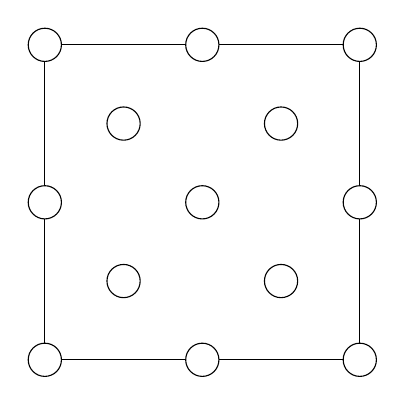
\begin{tikzpicture}
    \draw[-] (0,0) -- (4,0) -- (4,4) -- (0,4) -- (0,0);
    \filldraw[fill=white, draw=black] (0,0) circle (6pt);
    \filldraw[fill=white, draw=black] (4,0) circle (6pt);
    \filldraw[fill=white, draw=black] (0,4) circle (6pt);
    \filldraw[fill=white, draw=black] (4,4) circle (6pt);
    \filldraw[fill=white, draw=black] (0,2) circle (6pt);
    \filldraw[fill=white, draw=black] (2,2) circle (6pt);
    \filldraw[fill=white, draw=black] (2,0) circle (6pt);
    \filldraw[fill=white, draw=black] (4,2) circle (6pt);
    \filldraw[fill=white, draw=black] (2,4) circle (6pt);
    \filldraw[fill=white, draw=black] (1,3) circle (6pt);
    \filldraw[fill=white, draw=black] (1,1) circle (6pt);
    \filldraw[fill=white, draw=black] (3,3) circle (6pt);
    \filldraw[fill=white, draw=black] (3,1) circle (6pt);
\end{tikzpicture}
\end{document}